\documentclass[a4paper,man,natbib]{apa6}

\usepackage[english]{babel}
\usepackage[utf8x]{inputenc}
\usepackage{amsmath}
\usepackage{graphicx}
\usepackage[colorinlistoftodos]{todonotes}

\usepackage{verbatim}
\usepackage{placeins}
\usepackage{float}
\restylefloat{figure}
\restylefloat{table}

\usepackage{tikz}
\usetikzlibrary{shapes,arrows}


\title{Troubleshooting and Diagnostic Analysis of Earth-mover Scraper --- CAT 637}
\shorttitle{CAT 637G --- troubleshooting analysis }
\author{Prepared for

Lisa Slywka, Instructor

English and Communications

School of Applied Sciences and Technology
}
\affiliation{Prepared by

Tai Tran, 200222333

Industrial Heavy Equipment Technician Program

School of Applied Trades

October 31, 2016
}

% \abstract{Your abstract here.}
    
\begin{comment}
%%%%%%%%%%%%%%%%%%%%%%%%%%%%%%%%%%%%%%%%%%%%%%%%%%%%%%%%%%%%%

You can add inline TODO comments with the todonotes package, like this:
\todo[inline, color=green!40]{This is an inline comment.}

% refer to table %%%%%%%%%%%%%%%%%%%%%%%%%%%
\ref{tab:widgets}

% mathematics %%%%%%%%%%%%%%%%%%%%%%%%%%%%
\LaTeX{} is great at typesetting mathematics. Let $X_1, X_2, \ldots, X_n$ be a sequence of independent and identically distributed random variables with $\text{E}[X_i] = \mu$ and $\text{Var}[X_i] = \sigma^2 < \infty$, and let
$$S_n = \frac{X_1 + X_2 + \cdots + X_n}{n} = \frac{1}{n}\sum_{i}^{n} X_i$$
denote their mean. Then as $n$ approaches infinity, the random variables $\sqrt{n}(S_n - \mu)$ converge in distribution to a normal $\mathcal{N}(0, \sigma^2)$.

% lists %%%%%%%%%%%%%%%%%%%%%%%%%%%%
\begin{enumerate}
\item Like this,
\item and like this.
\end{enumerate}
\dots or bullet points \dots
\begin{itemize}
\item Like this,
\item and like this.
\end{itemize}

%%%%%%%%%%%%%%%%%%%%%%%%%%%%%%%%%%%%%%%%%%%%%%%%%%%%%%%%%%%%%
\end{comment}

\begin{document}

\centering The Northern Alberta Institute of Technology\\ Edmonton, Alberta

\maketitle

\tableofcontents
\newpage

\listoffigures
\newpage

\listoftables
\newpage



\section{INTRODUCTION}

\subsection{The Significant of Troubleshooting Analysis}

Cutting cost, reducing downtime, and extending lifespan of equipment are some business goals in the heavy equipment industry. In order to meet these targets, preventative maintenance can be the best practice; however, depending on environment and workload, equipment can fail at any time between service intervals. For this reason, technicians must equip themselves with appropriate troubleshooting skills.

Hydraulics are a main focus in the heavy equipment maintenance world. Likewise, in CAT 637G, hydraulics are also used in many places, including cushion-hitch, auger, push-pull hydraulic systems. Despite of versatile abilities, hydraulic systems are susceptible to contamination since components are usually exposed to dusty environments. Compared to other hydraulic systems, the powertrain might less prone to contamination since its components are less exposed. Therefore, their service life may be longer than other hydraulic systems, but failures can cause longer downtime. This research will provide some diagnostic instructions to solve hydraulic systems and powertrain issues.

Understanding how to solve hydraulic and powertrain problems benefits both equipment owners and technicians. The ability to keep equipment in shape helps companies save money for other business goals and builds their reputation. As the vast majority of equipment heavily depends on hydraulics to do the job, including powertrain, technicians or students with troubleshooting skill in this field can consolidate their positions or increase the chances of getting a good job.

\subsection{Scope}

As the paper has word limitation, the research will cover basic diagnostic instructions for common hydraulics and powertrain issues of CAT 637G. Typically, the focused areas of hydraulics are the cushion-hitch circuit and general hydraulic systems, while the focused area of powertrain is only the torque converter. Besides, this paper also includes some safety measures as a part of troubleshooting procedures.

\section{EQUIPMENT DESCRIPTION}
\label{sec:examples}

\subsection{History Background}
 
Back in 1922, Robert Gilmour Letourneau and his brother-in-law Ray Peterson built the first earthmoving scraper in Stockton, California \citep[p. 35]{RLMBldng}. After the first scraper was built by Letourneau in 1922, the author created a second version of earthmoving scraper, nicknamed the Gondola. Later, the third edition Mountain Mover was created in 1923. The Self-Propelled scraper was the fourth built. Letourneau continuously dedicated his life to improve his creations \citep{RLMBldng}.

\begin{figure}[!ht]
\centering
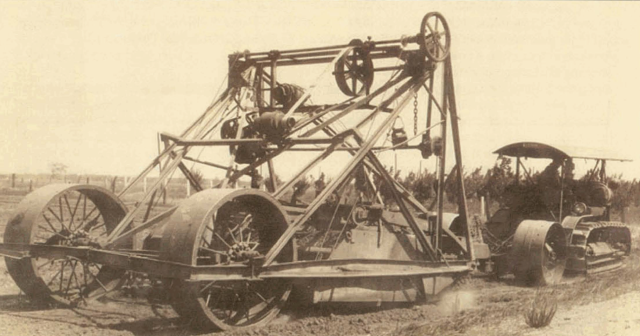
\includegraphics[width=0.5\textwidth]{mountain_mover_1922.png}
\centering\caption{\label{fig:rthcr1}Mountain Mover with a telescoping bowl was invented in June, 1922. \citep{RLMBldng}}
\end{figure}

\subsection{Components}

\section{Diagnostics and Troubleshooting Analysis}

\subsection{Hydraulic Systems}

\subsubsection{Cushion-hitch Hydraulic System}

\subsubsection{Auger Hydraulic System}

\subsection{Powertrain}

\subsubsection{Torque Converter}

\section{CONCLUSION}

\bibliography{main}

\end{document}


